\chapter{Цифровой двойник сетевых физических процессов}\label{ch:ch6}

\subsubsection{6.1.1}

This paper demonstrates the power of big data analysis of social media for the identification and prioritization of supply chain risks in clothing industry. Due to their high volume, data from social media can be considered a good source for obtaining customer feedback. On the other hand, the high volume of social media data could be efficiently processed solely by special tools for big data analysis. Results of such an analysis include clusters of words, topics and sentiments which allow decision makers to gather negative customer feedback and to manage risks in the distribution of products. A case study in the segment of footwear supply chain was analyzed, where one month of data from Twitter was used.

\subsubsection{6.3.1}

In this research, the authors consider methods for identifying geodata of users of social networks within user discussions. The knowledge of user geolocation data makes it possible to analyze the spread of discussion among users of different countries. Authors do not try to determine the exact geolocation, but rather the country where the users are located. The problem of getting country-level user location data lies in the fact that a high percentage of users do not state their location correctly, either mentioning it in humorous ways or even not stating it at all. There are various methods of obtaining data about the location of users. Among them, there are text-based methods, methods based on the analysis of the context, and methods based on the topology of the user graph. In this paper, we make a special emphasis on a method that allows to reveal geodata of users who specified their geodata incorrectly or did not specify it at all. In order to test our method, we use Twitter datasets.

\section{Цепь поставок}\label{sec:ch6/sect1}

\subsection{Big Data Analysis in Social Networks for Managing Risks}\label{subsec:ch6/sec1/sub1}

\paragraph{Introduction.} Nowadays clothing industry contributes noticeably to world-wide economy. Herewith large textile corporations sell primarily brands, not clothes itself. Thus, the main value for the modern clothing industry giants is a favourable consumer attitude \cite{Choi}. es itself. Hence, one of the main risks in the clothing industry is associated with the loss of confidence caused by negative feedback of customers \cite{IvanovDolguiSokolovIvanova,ChiuChoiDai}. Efficient risk management in such a field stems from analysis of consumer’s activities in social media \cite{Choi}. Indeed, deep analysis of activities in social media can enable decision-makers to obtain clear information on different risk aspects associated with a product that may cause a negative response from customers. Eventually, customer dissatisfaction may lead to a brand change. Mass brand reject may lead to financial loss and even bankruptcy of a textiles corporation \cite{TianChoiDing}.

Big data has been characterized in literature by 5Vs: volume, variety, velocity, veracity and value \cite{GunasekaranTiwariDubey}. Veracity and value are particularly important since data analysis shows the real value of big data. Big data analytics (BDA) is based on knowledge extraction from vast amounts of data, facilitating data-driven decision-making.

BDA has been undoubtedly the most elaborated area of digital technologies application to supply chain management over the last decade. Simchi-Levi and Wu \cite{SimchiLeviWu} analysed the application of BDA to retail and concluded that retailers must continuously strive to grow their revenue, margins and market share. Nguyen et al. \cite{NguyenZhouSpiegler} showed that optimization is the most popular approach in prescriptive analytics application to logistics and transportation area.

BDA applications to supply chain management can also be seen in procurement processes, manufacturing shop floors, promotion actions in the omnichannel model, routing optimization, real-time traffic operation monitoring and proactive safety management \cite{GunasekaranTiwariDubey,NguyenZhouSpiegler}. Papadopoulos et al. \cite{PapadopoulosGunasekaranDubey} pointed out that BDA can help in improving SC risk management and disasterresistance. Dolgui et al. \cite{DolguiIvanovSokolov} and Ivanov \cite{Ivanov} identified frameworks of risk management in the supply chains using digital technologies and data analytics.

Recent relevant implementation of big data analysis in social media (Twitter) to industry was made by Singh et al. \cite{SinghShuklaMishra}. They considered food industry and developed the approach which could inform supply chain decision-makers about customer feedback and issues in the flow/quality of food products.

Twitter information seems to be one of the most widely used data source for research and applications (see, for instance, \cite{ChenElmesChang} and \cite{BodrunovaLitvinenkoBlekanov}). In the context of brand management Twitter information was considered by Malhotra et al. \cite{MalhotraMalhotraSee}. Utilization of Twitter data is expanding in numerous directions from market prediction to public safety. Analysis of Twitter data has also been conducted by researchers in the domain of operation management \cite{TanZhanJi,FanNiu}.

This paper is devoted to investigation of Twitter information as an analytical basis for risk management in clothing industry. In particular, operational risks in the apparel supply chains are analysed which are usually concerned with demand and lead time fluctuations \cite{Ivanov,IvanovDolguiSokolov}.

\paragraph{Case study and Twitter data analysis.} The Twitter data analyzed in this research was used to understand issues related to risks identification in clothing supply chains. This analysis can help to illuminate reasons behind negative sentiments in discussions of Twitter users about sneakers. Sneakers are very popular footwear today which is discussed intensively. 

The total number of tweets extracted for this research was 248,728. They were captured from 01/09/2018 to 30/09/2018 using the keyword ‘sneakers’. Only tweets written in English language were considered, with no geographic constraint.

\begin{table} [htbp]%
	\centering
	\caption{Size of the discussion.}%
	\label{tab:discussionSize}% label всегда желательно идти после caption
	\renewcommand{\arraystretch}{1.6}%% Увеличение расстояния между рядами, для улучшения восприятия.
		\begin{tabulary}{\textwidth}{@{}>{\zz}L >{\zz}C@{}}% Вертикальные полосы не используются принципиально, как и лишние горизонтальные (допускается по ГОСТ 2.105 пункт 4.4.5) % @{} позволяет прижиматься к краям
			\toprule     %%% верхняя линейка
			Number of tweets & 248,728 \\ 
			Number of likes & 748,887  \\
			Number of retweets & 159,141 \\ 
			Number of comments & 125,747 \\ 
			\bottomrule %%% нижняя линейка
		\end{tabulary}%
\end{table}

The scale of the discussion depends not only on a total number of tweets but also on the value of discussion based on reaction of Twitter users to the topic. Indeed, total number of tweets without reaction of Twitter users can be associated with information attack or unfair market competition. Conversely, large amount of likes, retweets and comments means a discussion is of interest in Twitter community.

According to Table~\cref{tab:discussionSize}, discussion on sneakers is initiated by 248,728 tweets and, what is really important, generates 1,282,503 of total actions by Twitter users during one month. No doubt that it is indicative discussion and could be used for informative analyses. Figure~\cref{fig:activityTypes} visualizes that main contribution in the discussion activities is made by likes. This fact should be taken into consideration very carefully by analysts.

\begin{figure}[ht]
	\centerfloat{
		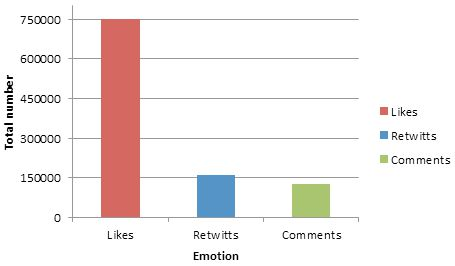
\includegraphics[scale=1.3]{activityTypes}
	}
	\caption{Types of activities.}\label{fig:activityTypes}
\end{figure}

Other important information to be extracted concerns number of real Twitter users involved in the discussion. This aspect is demonstrated in Table~\cref{tab:uniqueTwitterUsers}. Therefore, the discussion on sneakers in English-tweeting community during September of 2018 was initiated by 113,669 unique users, while 224,412 unique users take part in this discussion.

\begin{table} [htbp]%
	\centering
	\caption{Unique Twitter users.}%
	\label{tab:uniqueTwitterUsers}% label всегда желательно идти после caption
	\renewcommand{\arraystretch}{1.6}%% Увеличение расстояния между рядами, для улучшения восприятия.
	\begin{tabulary}{\textwidth}{@{}>{\zz}L >{\zz}C@{}}% Вертикальные полосы не используются принципиально, как и лишние горизонтальные (допускается по ГОСТ 2.105 пункт 4.4.5) % @{} позволяет прижиматься к краям
		\toprule     %%% верхняя линейка
		Number of unique tweeting users & 113,669 \\ 
		Number of unique users in the discussion & 224,412  \\
		\bottomrule %%% нижняя линейка
	\end{tabulary}%
\end{table}

Figure~\cref{fig:dailyTweetDynamics} demonstrates the dynamics of daily tweets devoted to sneakers during the September of 2018. The dynamics of the discussion has the peak in the beginning of month and then shows average fluctuation.

\begin{figure}[ht]
	\centerfloat{
		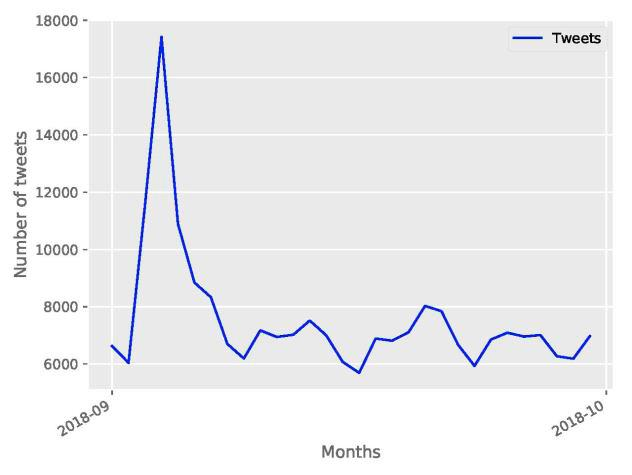
\includegraphics[scale=1]{dailyTweetDynamics}
	}
	\caption{Dynamics of daily tweets on sneakers in September 2018.}\label{fig:dailyTweetDynamics}
\end{figure}

Several hashtags were observed in the collected tweets. The most frequently used hashtags are highlighted in Table~\cref{tab:topHastags}.

\begin{table} [htbp]%
	\centering
	\caption{Top hashtags used.}%
	\label{tab:topHastags}% label всегда желательно идти после caption
	\renewcommand{\arraystretch}{1.6}%% Увеличение расстояния между рядами, для улучшения восприятия.
	\begin{adjustbox}{width=0.29\textwidth}
		\small
		\begin{tabulary}{\textwidth}{@{}>{\zz}L >{\zz}C >{\zz}C@{}}% Вертикальные полосы не используются принципиально, как и лишние горизонтальные (допускается по ГОСТ 2.105 пункт 4.4.5) % @{} позволяет прижиматься к краям
			\toprule     %%% верхняя линейка
			Hashtag & Freq (>100) & Freq(\%) \\
			\midrule %%% тонкий разделитель. Отделяет названия столбцов. Обязателен по ГОСТ 2.105 пункт 4.4.5
			\#sneakers & 1987 & 49.69 \\ 
			\#nike & 1077 & 26.93 \\
			\#sneakerhead & 680 & 17.00 \\ 
			\#kicks & 444 & 11.10 \\ 
			\#sneakerheads & 374 & 9.35 \\
			\#shoes & 343 & 8.58 \\
			\#sneaker & 331 & 8.28   \\ 
			\#kicksonfire & 322 & 8.05  \\
			\#jordan & 299 & 7.48 \\
			\#kotd & 269 & 6.73 \\ 
			\#airmax & 260 & 6.50 \\
			\#backtoschoolpic & 241 & 6.03 \\ 
			\#sneakeraddict & 241 & 6.03 \\
			\#athleisure & 227 & 5.68 \\
			\#ootd & 224 & 5.60 \\ 
			\#air & 211 & 5.28 \\
			\#sneakerfreak & 206 & 5.15 \\
			\#fashion & 195 & 4.88 \\
			\#airjordan & 195 & 4.88 \\
			\#sneakerfreaker & 184 & 4.60 \\
			\#shopmycloset & 161 & 4.03 \\
			\#soleretriever & 158 & 3.95 \\
			\#adidas & 157 & 3.93 \\
			\#mensfashion & 152 & 3.80 \\
			\#hypebeast & 148 & 3.70 \\
			\#sneakershopping & 138 & 3.45 \\
			\#sepatu & 124 & 3.10 \\
			\#lifestyle & 123 & 3.01 \\
			\#yeezy & 122 & 3.05 \\
			 \#fashionista & 121 & 3.03 \\
			\bottomrule %%% нижняя линейка
		\end{tabulary}%
	\end{adjustbox}
\end{table}

Keyword and hashtags allow for information accumulation on the topic. Hashtags demonstrate bright points of discussions. Herewith, a tweet consists of several words and carries semantic content. Big data analysis tool allows us to extract most frequently used words in tweets from considered set (table~\cref{tab:wordsUsed}).

\begin{table} [htbp]%
	\centering
	\caption{Words used in extracted tweets.}%
	\label{tab:wordsUsed}% label всегда желательно идти после caption
	\renewcommand{\arraystretch}{1.6}%% Увеличение расстояния между рядами, для улучшения восприятия.
	\begin{adjustbox}{width=0.25\textwidth}
		\small
		\begin{tabulary}{\textwidth}{@{}>{\zz}L >{\zz}C >{\zz}C@{}}% Вертикальные полосы не используются принципиально, как и лишние горизонтальные (допускается по ГОСТ 2.105 пункт 4.4.5) % @{} позволяет прижиматься к краям
			\toprule     %%% верхняя линейка
			Hashtag & Freq (>500) & Freq(\%) \\
			\midrule %%% тонкий разделитель. Отделяет названия столбцов. Обязателен по ГОСТ 2.105 пункт 4.4.5
			air & 9740 & 32.88 \\
			sneakers & 9657 & 32.60 \\
			nike & 6711 & 22.66 \\
			sneaker & 3385 & 11.43  \\
			max & 3147 & 10.62 \\
			jordan & 3128 & 10.56 \\
			mens & 2387 & 8.06 \\
			shoes & 2097 & 7.08 \\
			size & 1797 & 6.07 \\
			new & 1628 & 5.50 \\
			retro & 1382 & 4.67 \\
			white & 1209 & 4.08 \\
			black & 1118 & 3.77 \\
			force & 1048 & 3.54 \\
			running & 1005 & 3.40 \\
			ya & 971 & 3.28 \\   
			us & 873 & 2.95 \\
			di & 824 & 2.78 \\
			just & 792 & 2.67 \\
			via & 752 & 2.54 \\
			x & 729 & 2.46 \\
			now & 713 & 2.41 \\
			sneakerhead & 695 & 2.35 \\
			fashion & 687 & 2.32 \\
			ebay & 638 & 2.15 \\
			athletic & 628 & 2.12 \\
			amp & 607 & 2.05 \\
			check & 605 & 2.04 \\
			available & 594 & 2.01 \\
			brand & 593 & 2.00 \\			
			\bottomrule %%% нижняя линейка
		\end{tabulary}%
	\end{adjustbox}
\end{table}

Words extracted from tweets about sneakers occur in different combinations. Intellectual analysis, based on Biterm Topic Model, revealed seven macro topics which generate discussions \cite{BlekanovTarasovMaksimov}. Biterm Topic Model helps analysing a set of biterms (i.e., unordered word pair co-occurring in a short context). The main idea is that if two words co-occur more frequently, they are more likely to belong to a same topic \cite{YanyanJiafengXueqi}. Btm assumes the following generative process:
\begin{itemize}
	\item first, we draw distribution of tweets’ topics by distribution of Dirichlet,
	\item second, for each topic:
	\begin{itemize}
		\item we draw distribution of topics’ words by multino- mial distribution,
	\end{itemize}
	\item third, for each biterm:
	\begin{itemize}
		\item we draw distribution of biterms by multinomial
		distribution,
		\item we draw distribution of each term in this biterm separate multinomial distributions.
	\end{itemize}
\end{itemize}

As BTM does not model tweets explicitly, we need to provide a way to infer the topics in a tweet, i.e., evaluating the topic posterior. In this regard, we developed the chain rule based on Bayes’ formula and empirical distribution of words in a tweet.

As a result of the analysis seven topics were defined. Topic 1 unfolded around men sneakers. Twitter users share information about sizes and models, give positive and negative comments on the topic. Topics 2 and 3 can be characterized as meta-topics -- topics that do not contain any sense but express some artificially established patterns of the words. Topic 4 generates discussions around such model of sneakers as air. Topic 5 generates discussions around sales of amp and air sneakers. Topics 6 and 7 seem to be meta-topics too. Hot map of revealed topics is given in figure~\cref{fig:topicHotMap}.

\begin{figure}[ht]
	\centerfloat{
		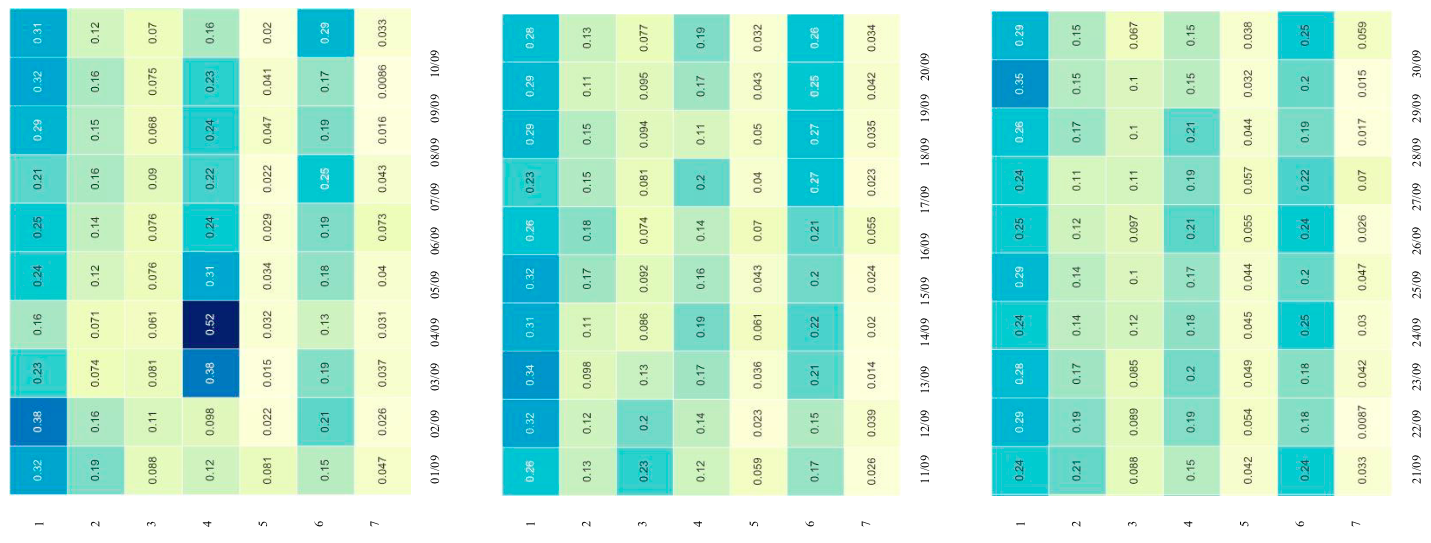
\includegraphics[angle=270, scale=0.5]{topicHotMap}
	}
	\caption{Hot map of topics devoted to sneakers in September 2018.}\label{fig:topicHotMap}
\end{figure}

From risk management perspectives negative tweets should be drifted apart from all others and analysed separately. During September of 2018 there were posted 14,181 negative tweets. Dynamic of negative tweets is given by figure~\cref{fig:dailyNegativeTweetDynamics}. Peak of negative feedback and hot discussion on topic 4 has direct correlation. Indeed, both peaks occur in the beginning of September. Therefore, it could be concluded that customers gave negative feedback in the beginning of September on topic 4. Semantic analysis defined that the main cause lies in disappointed expectation of customers. More precisely, new air sneakers were expected to be released but this did not happen (maybe customers just did not have accurate information on that). Anyway this caused irritation among customers that can be easily observed in many tweets. Thus, risk managers should take this situation into consideration and recommend to decision-makers to prevent leaks of information about new releases or make official statements in this regard in “on-line” regime.

\begin{figure}[ht]
	\centerfloat{
		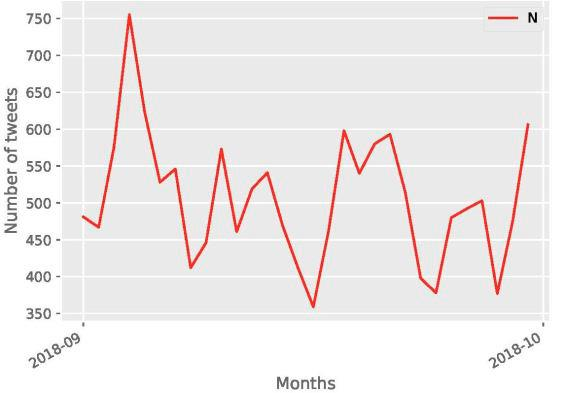
\includegraphics[scale=1.0]{dailyNegativeTweetDynamics}
	}
	\caption{Dynamic of daily negative tweets devoted to sneakers in September 2018.}\label{fig:dailyNegativeTweetDynamics}
\end{figure}

\paragraph{Managerial implications.} Social networks became insistently important source for different types of information. Nevertheless, the considered case study showed how much extended data analysis is required to establish informative issues for revealing risk points from Twitter. The investigated case study pertains to the following conclusion: textiles corporations should increase their presence in social networks to minimize operational risks. Therefore, in spite of its complexity big data analysis of social networks could be valuable source of information for risk managers and decision-makers at different levels in textiles industry.

\paragraph{Conclusion.} Social networks are increasingly affecting various aspects of human life. Thus social networks also impact different economic processes. In this paper, the case study in the segment of footwear supply chain was analysed, where data from Twitter was used for a period of one month. Analysis showed that discussion contains more than one million activities in Twitter devoted to the considered keyword. Such amount of activities should not be ignored while minimizing risks in clothing distribution by textiles corporations. In future work we are planning to extend our research and investigate social network data analysis for longer period of times and a broad product range to contribute to decision-making support in supply chain risk management.

\section{Визуализация}\label{sec:ch6/sect2}

\section{Геопозиция}\label{sec:ch6/sect3}

\subsection{Geolocation Detection Approaches for User Discussion Analysis in Twitter}\label{subsec:ch6/sec3/sub1}

\subsubsection{1 Introduction}

Social media services on the Internet, such as microblogs offered by social media platforms such as Twitter, have demonstrated a phenomenal growth in the amount of users. This growth has sparked interest in using the data provided by these platforms to extract various kinds of information, such as, for example, the geographical location of users. The data obtained can be used to provide users with personalized services, such as relevant news, advertising, marketing and other content. Knowledge about the geolocation of users can allow researchers to analyze global social events in terms of which segments of the population they have influence on and what kind of influence there is. With over 300 million monthly active Twitter accounts in various geographical locations, the short messages they generate form a huge dataset that can be analyzed to extract such geographical information.

Twitter allows its users to specify their own geographical location. Location information is entered manually by the user or updated using GPS (but this function is activated only by small percentage of users \cite{ChengCaverleeLee} of the network). Consequently, geolocation data may be missing or incorrect for most users. There are several types of problems when using geolocation data, which are set and updated manually by users:

\begin{itemize}
	\item Limited access to the Twitter API. The only tool for obtaining information about the geolocation of users is the official Twitter API service. Unfortunately, since 2021, access to this service is opened exclusively on a paid basis.
	\item Incorrect user data. Users may enter incorrect or fictitious geographical location data. For example, a user can enter “Mars, Kowalski crater” as a geo-position. Also, users can use geographical locations that do not exist at all, for example, “Krypton”.
	\item Data ambiguity. Some users ambiguously indicate geolocation information. For example, “cosmopolitan, but from Moscow”. It is difficult to process such a string with a naive approach, since there is a lot of unnecessary information in it;
	\item Lack of user geodata.
\end{itemize}

\subsubsection{2 Related works}

Various approaches are used to solve the problem of the availability of information about the geolocation of users. They can be divided into 3 classes:
\begin{enumerate}
	\item Methods based on the text content of the message.
	\item Methods based on connections in the social graph of users.
	\item Methods based on the context of user messages.
\end{enumerate}

\paragraph{2.1 Methods based on the text content of the message} This class of methods includes approaches that use information about dialects, which are aimed at finding and using special words to determine the geolocation of users. Obviously, not all words indicate geolocation. Therefore, only local words should be used, i.e. words that are used by users living in the same territory and indicating their geolocation.

According to statistics, local words that can be used to identify a geo-location are much less common in the text than the usual frequently used words. Methods of identifying local words without a teacher are aimed at calculating statistical indicators. So, using the idea of the Inverse Document Frequency (IDF) indicator \cite{RenZhangLin,HanCookBaldwin,MahmudNicholsDrews2014} propose Inverse Location Frequency (ILF) and Inverse City Frequency (ICF), respectively, to measure the locality of words. Usage of such idea minimizes the use and spread of local words by increasing the values of ILF and ICF. Authors \cite{MahmudNicholsDrews} applied a number of heuristic rules to select local words. In the research \cite{HanCookBaldwin2014}, the authors propose a comparison of statistical methods based on information theory and heuristic methods for selecting local words.

Methods of identifying local words with a teacher are also considered in a number of studies. In studies \cite{ChengCaverleeLee}, the problem of searching for local words was considered as a classification problem. First, the authors construct the geographical distribution of each word using a spatial variation model presented by authors in \cite{BackstromKleinbergKumar}. The spatial variation model assumes that each word has a geographical center, a central frequency and a coefficient of variance. The probability of using a word together with the distance to the center is proportional to the central frequency. Then the authors manually marked up 19178 words from the dictionary into local and non-local ones. As a result, a trained classifier was obtained, which the authors applied to the rest of the words from the marked-up list. The authors of the article \cite{RyooMoon} applied the above method and achieved satisfactory results for a set of Twitter messages in Korean.

After identifying local words, the next problem is to use them to predict the geolocation of users. Most researchers propose probabilistic models for constructing the distribution of users by geolocation, using the textual context of their messages, and then concretize the model for forecasting \cite{ChengCaverleeLee}. Another approach is based on highlighting local words of a special type in the message text, such words are the names of places. Authors \cite{LiWangChang} noticed that the probability of mentioning place names in messages can be both natural and depend on geolocation, and be random. Thus, the authors make a two-level assessment based on the Bernoulli distribution of randomness or regularity of mentioning the name of a place to determine geolocation and a polynomial distribution to estimate the probability of publishing a message with the name of a place from each geolocation.

In several studies, classification methods are used to detect and predict the location of users. Researchers consider user statistics on the use of local words in communications as signs, and various geolocations as classification labels. B. Hecht et al. \cite{HechtHongSuh} choose 10,000 words with the highest CALGARI scores as local words. Then users are represented as 10000-dimensional vectors with the values of the frequencies of terms, which are fed into the naive Bayesian classifier for training and predicting the geolocation of users. Similarly, Rahimi et al. \cite{RahimiVuCohn} apply logistic regression to TF-IDF vectors of users. Instead of using local words as features, the authors add constraints using L1-regularization. In \cite{MahmudNicholsDrews,MahmudNicholsDrews2014} authors apply a hierarchical ensemble of algorithms to train ensembles of two-level classifiers to determine a geo-location with varying degrees of detail, such as a city, state, or time zone.

There are also studies in which approaches based on information analysis are used to determine the geolocation of users. In this case, locations are treated as pseudo-documents consisting of tweets from all users living in this location. Considering the pseudo-document of the user whose geolocation needs to be predicted, the most similar pseudo-documents are issued as the results of forecasting. In particular, \cite{WingBaldridge} represent geolocation in the form of a grid. The authors evaluate the language model for each grid with its pseudo-document. In other studies \cite{RollerSperiosuRallapalli}, the authors use the Kullback-Leibler distance as a measure of similarity between geolocation pseudo-documents and user pseudo-documents. In their subsequent work \cite{WingBaldridge2014}, the authors use adaptive networks.

In addition to traditional methods, some papers also explore deep learning models for predicting user geolocation. Continuing their previous work \cite{MiuraTaniguchiTaniguchi,MiuraTaniguchiTaniguchi2017} authors propose a more complex model. The authors organize the Twitter user's messages in chronological order and apply a sequential RNN model for encoding. Thanks to the attention mechanism, it is possible to get a general idea of the message, which contains important and necessary information. A similar process can also be applied to context, i.e. to the description of the geodata of the message and the time zone. Then the combination of the three representations is passed to the softmax layer to determine the geolocation of the user. In \cite{RahimiCohnBaldwin} authors use a multilayer perceptron (MLP) with one hidden layer to classify user geolocation. The authors use the representation of the user's message in the form of an L2-normalized bag of words as input. The output is a predefined discretized region generated either by a k-d tree or by a k-means algorithm.

\paragraph{2.2 Methods based on links in the social graph of users} In addition to generating content, users of social networks, in particular Twitter, perform other interesting activities, the analysis of which helps to reveal hidden patterns that have a positive impact on the definition of geolocation of users. Such activities include, for example, the subscription of some users to the accounts of others, the establishment of friendly relations between users, the reaction of some users to the published content of others through tools built into the social network, such as "likes", reposts and comments. Like the content of user messages, users' social relationships on social networks can also indicate their geo-location.

Such relationships are described in sociology by the concept of “homophilia”, which indicates the tendency of individuals to be more likely to come into contact with people similar to them. Considering this concept in the context of the task of detecting the geolocation of users, the user's location most likely coincides with the geolocation of most of his friends. Authors \cite{RenZhangLin} suggested that the more friends a user has in a particular place, the higher is the probability that the user is in the same location. \cite{DavisPappaDeOliveira} use a similar approach, except that they consider only mutual friendship. All the methods mentioned above implicitly assume that friendly relations between users on a social network implies friendship in real life and, consequently, a small distance between the geolocations of friends. However, this may be far from the truth. In studies \cite{KongLiuHuang}, the authors found that a couple of friends live within 10 km with a probability of 83\% if their mutual friends make up more than half of the entire list of their friends. The probability is reduced to 2.4\% if the number of common friends is 10\%. This means that a strong friendship based on the total number of users' friends can better indicate friendship in real life and positively influence the proximity of their geolocations.

In social networks, mention is another type of user interaction. When users mention each other in a discussion, it is assumed that such users have similar interests. Information about this type of friendship is very useful for determining the geo-positions of users. McGee et al. \cite{McGeeCaverleeCheng} conducted an analysis of 104214 users living in the USA. The authors found out that in addition to mutual friendship based on subscriptions, mentions and conversations of users also indicate a small distance between their geolocations. In his next paper, McGee et al. \cite{McGeeCaverleeCheng2013} confirmed their observations by examining a more extensive data set. Other observations were also noted:
\begin{enumerate}
	\item if the user's subscriber account is closed, i.e. other users need permission to subscribe to this account, then these two users are located close to each other;
	\item accounts of local news sources are located in the same location with their subscribers.
\end{enumerate}

Considering geographical proximity to be directly related to social proximity \cite{McGeeCaverleeCheng2013} trained a decision tree to compare social proximity between different users to ten quantiles. As well as \cite{McGeeCaverleeCheng,McGeeCaverleeCheng2013}, Compton et al. in \cite{ComptonJurgensAllen} also use information about the mention of users in the text content of the message. The authors build a graph of user mentions and identify unknown locations so that users mentioning each other are close to each other. In studies \cite{Jurgens}, authors also consider mutual mentions of users as friendships. Rahimi et al. in \cite{RahimiCohnBaldwin} argue that mutual mentions are too rare to be useful. The authors consider the mention by one user of another as an undirected edge in the graph.

\paragraph{2.3 Methods based on the context of user messages} Authors \cite{MahmudNicholsDrews,MahmudNicholsDrews2014} take into account the time of publication of the tweet, the values of which are presented in GMT format in the dataset under consideration. After dividing the day into time intervals of equal length, users are considered as distributions of the publication time of their messages. Then, when using the classifier, the shifts of distributions caused by the difference in time zones are also taken into account. In other studies \cite{EfstathiadesAntoniadesPallis} authors use a probabilistic model based on the time distribution of geographical labels of text messages to estimate the location of the user's home and workplace. The method is based on the authors’ observation that the publication of messages by the user during non-working hours (for example, in the evening) is most likely to occur from the "home" geolocation, while the publication of posts during working hours is most likely to occur from the working location. Authors \cite{PoulstonStevensonBontcheva} also use geotags in their work, but note the publication activity of users in several locations at once. The authors first cluster geotags, and then define the group with the largest number of posts as a “home’ geolocation. The geometric median of all points in the “home cluster” is taken as the coordinates of the “home” geolocation.

\paragraph{2.4 Summary} Thus, different methods of analysis and forecasting are used to detect the geolocation of users. More accurate geolocation detection models are based on combined approaches using both the text content of user messages and information about the structural interaction of users. The use of such a number of diverse content parameters has a positive effect on the accuracy of detection, however, it negatively affects the speed of calculations, and in some cases, the inability to use individual parts of the content due to the privacy settings of the user's profile in the social network. The speed problem is especially sensitive when processing user discussions in social networks within the framework of real events, where the volume of discussion can vary greatly even over a short period of analysis (from tens of thousands of users to several million). Therefore, as part of the implementation of the current stage, exceptionally fast methods of detecting user geolocation were considered.

\subsubsection{3 Our approach for user geolocation detection in Twitter discussions}

To implement our software solution for determining geolocation, a micro-service architecture was chosen, which allows us to present each stage of data processing as a separate service. This approach ensures the modularity of the system, which makes it possible to distribute tasks more efficiently and structure work on the solution.

To solve the problem of accessibility of information about the geolocation of users, it was decided to evaluate the geographical position of a Twitter user at the level of him belonging to the country. The following types of information were used as source data:

\begin{itemize}
	\item information specified by the user on his personal Twitter page in a special localization field. It contains text string of limited length.
	\item information about the structural interaction of users of the discussion with each other through built-in tools (such as "likes", reposts, comments). This discussion information is presented in the form of a user-oriented web graph described in the hidden communities search section.
\end{itemize}

\paragraph{3.1 Discussion processing} The discussion processing consists of several stages:
\begin{enumerate}
	\item obtaining the geolocation information specified by the user in accordance with his unique name. This information was collected and processed using a search robot developed previously for working with Twitter data.
	\item processing of the received information with a naive OSM or naïve approach (Open Street Maps API). With the help of the search robot in the previous step, text information was extracted from a special location field for each user of the discussion. The received list of text strings with a potential geolocation name at this stage is verified using the program API of the non-commercial web mapping project Open Street Maps (OSM), Nominatim in particular. It is a tool for searching OSM data by name and address of a geographical location. Nominatim accepts a string with the name of the object as input and, in case of successful verification, returns a JSON containing the two-letter code of the country in which the object is located. The resulting code is further reduced to the standard form in ISO 3 with the help of a dependency dictionary. It is important to note that each processed string is saved to the database in order to minimize the frequency of API requests in case it has multiple occurrences.
	\item improving the results of the previous step by using named entity recognition methods “naïve+NER”. As noted in the review, in real life, users more often enter their location randomly, without any particular pattern, which leads to the fact that this data cannot be processed using just OSM Nominatim. Let's take “I'm from St. Petersburg” as an example of a string. Processing this string using the API will return an error. However, OSM Nominatim returns a correct result ‘ru’ for the "Saint Petersburg" string. This problem of geodata noise is solved using Named Entity Recognition methods (hereinafter referred to as NER). The python spaCy library was considered as a ready implementation of NER for this project. NER allows not only to define named entities, but also to assign them to one of the following labels:
	\begin{itemize}
		\item LOC (Location) - the name of the location (city, country, region, etc.);
		\item ORG (Organization) - the name of the organization;
		\item PER (Person) - first name, last name, etc.;
		\item MISC (Miscellaneous entities) - other various names (holidays, nationalities, products, works of art, etc.).
	\end{itemize}
	Pipeline of text processing in the case of spaCy is Transition-based NER . This architecture is described in the article \cite{DaiKarimiHachey}. The idea is as follows. We have a buffer of words in a sentence and an array of state words (initially empty). We also have operations on states: shift, reduce, out. Under these conditions, the task of NER is to predict the next operation. Matthew Honnibal, the creator of Explosion AI, one of the creators of spaCy, identifies four stages in named entity recognition algorithm:
	\begin{itemize}
		\item Embedding -- vectorization of document words;
		\item Encoding -- reduction of vectors obtained at the first stage to a matrix, where each row represents a layer in the context of the sentence under consideration;
		\item Vectorization (attend) -- bringing the sentence matrix obtained during the second stage to the form of a vector for further processing;
		\item Prediction -- classification of words in a sentence according to the received sentence vector.
	\end{itemize}
	As a result of the processing described above, we will get the source text with the labels of the recognized named entities. The LOC label is of particular interest for our task. It allows you to highlight geolocation in the user's noisy text. Thus, at this stage, the NER method is applied to the geolocation field. It searches for a word in the noisy text indicating geolocation, which is subsequently fed to OSM Nominatim.
	\item Determination of the remaining geolocations using the user discussion graph “naïve+NER+UserGraph”. The user graph was constructed according to the methodology proposed in the article \cite{BlekanovBodrunovaAkhmetov}. As a result of data processing at stage 2) and 3), two types of fields remain unprocessed at this stage:
	\begin{itemize}
		\item fields that do not contain information about the user's geolocation;
		\item empty/unfilled fields.
	\end{itemize}
	At this stage, information about the structural interaction of users in the discussion is taken into account. Using the glossary method, we assign users the geolocations that are most frequent among the participants of the discussion they mostly interact with. This approach does not allow to determine the true geolocation of the user, however, it reveals the probability of him choosing the side that he adheres to and quotes. Ideally, this approach calculates geolocation for each user of the discussion. However, it is important to note that the geolocation of some users may not be recognized in the following cases:
	\begin{itemize}
		\item the case of complete isolation of the vertex of the user web graph (when the user generated content but did not interact with other users);
		\item the case of partial isolation of the vertex of the user web graph (when the user has only one outgoing connection with another user);
		\item the case of mixed interaction of a vertex with two or more vertices (when the user has an equal number of outgoing connections with 2 (or more) users with different geolocations);
		\item the case of a vertex being connected exclusively with unidentified vertices (when the user does not have direct connections with identified vertices).
	\end{itemize}
\end{enumerate}

\paragraph{3.2 Datasets and evaluation measures} To evaluate the efficiency of the proposed approaches in relation to the task of determining the geolocation of users, several datasets of conflictual public discussions in Twitter were selected. These cases were collected from Twitter and studied by the authors in their previous papers \cite{BodrunovaLitvinenkoBlekanov,BodrunovaBlekanov,BodrunovaBlekanovSmoliarova}. The datasets of varying volumes were chosen to test the methods. The sample cases include the following datasets of different volumes:

\begin{itemize}
	\item a small user discussion (up to 10 thousand nodes) is a case of “Biryulevo”, which consists of tweets published on 17-31.10.2013 during the acute phase of unrest in the Moscow district of Western Biryulevo. Initially, it contains 11,429 users and 1,016 user connections. After excluding vertices with full, partial isolation and mixed vertices, there were 8670 users left.
	\item medium-sized user discussion (up to 50 thousand nodes) -- the “Keln” case contains data collected from 01 to 31.01.2016 as part of the discussion of mass attacks on women in Keln on the eve of 2016. Initially, it contained 40117 users and 98508 user links. After excluding vertices with full, partial isolation and mixed vertices, there were 30641 users left.
	\item large user discussion (up to 200 thousand nodes) -- the “Ferguson” case contains data from August 22 to 31, 2014 on riots in Ferguson provoked by the murder of an 18-year-old teenager by a policeman. Initially, it contained 169,676 users and 325,369 user connections. After excluding vertices with full, partial isolation and mixed vertices, 122779 users remained.
	\item extra-large user discussion (more than 500 thousand nodes) -- the case of “Charlie Hebdo” was retrieved for the period from January 7 to January 10, 2015 by collecting a response to a terrorist attack on the editorial office of Charlie Hebdo magazine. Initially, it contained 719503 users and 981131 user connections. After excluding vertices with full, partial isolation and mixed vertices, there were 580,580 users left.
\end{itemize}

We have introduced two measures in order to evaluate the proposed approaches. Recall-GEO (the number of users with determined geolocation divided by the total number of users) is used for all three methods, and the second one, Precision-GEO (the number users with properly detected geolocation divided by the total number of users with determined geolocation) is used for the UserGraph approach only.

A Recall-GEO completeness measure was used:
\[
\textit{Recall} - \textit{GEO} = \frac{\textit{number of users with identified geolocation}}{\textit{total number of users of the discussion}}
\]
To evaluate the accuracy of the graph algorithm, the following algorithm was used:
\begin{enumerate}
	\item Users were selected from real datasets, the ones who correctly indicated their geo-location, where the correctness was checked by OSM. As noted above, there is 55-59\% of the total number of such users ().
	\item The algorithm is first run on a data set with all the geolocations defined in the previous stages;
	\item Users with complete and partial isolation were removed from the obtained subsample of data.
	\item The resulting subsample was divided into a training and a test sample in a percentage ratio of 80\% and 20\%, respectively. The graph algorithm was run on a training sample, and the geolocation of users was calculated on a test sample.
	\item The results obtained are evaluated using the Precision-GEO accuracy measure: \[
	\textit{Precision} - \textit{GEO} = \frac{\textit{number of correct solutions}}{\textit{total number of solutions}}
	\]
\end{enumerate}

\paragraph{3.3 Evaluation results} The Table~\cref{tab:precisionGEOValues1} shows that in all 4 real discussions, 55--59\% of all users indicate their geolocation on their personal page. It is not difficult to notice that the proposed method of detecting the geolocation of users based on the recognition of named entities NER adds 7--12\% to the naive OSM approach. The graph method gives an increase of about 33\% on top of OSM on average and about 21\% on top of NER.

\begin{table}[ht]%
	\centering
	\caption{Precision-GEO measures values for four datasets}%
	\label{tab:precisionGEOValues1}% label всегда желательно идти после caption
		\begin{tabular}{ c  c  c  c  c }% Вертикальные полосы не используются принципиально, как и лишние горизонтальные (допускается по ГОСТ 2.105 пункт 4.4.5) % @{} позволяет прижиматься к краям
			\toprule
			Methods & Biryulevo & Köln & Ferguson & Charlie Hebdo\\
			\hline
			Total amount of users & 8670 & 30641 & 122779 & 580580\\
			naïve & 0,56 & 0,55 & 0,59 & 0,59\\
			naïve+NER & 0,60 & 0,61 & 0,65 & 0,66\\
			naïve+NER+UserGraph & 0,74 & 0,74 & 0,78 & 0,79\\
			\bottomrule
		\end{tabular}%
\end{table}

As a result of applying the Precision-GEO estimate described above on real user discussions, the following values were obtained (Table~\cref{tab:precisionGEOValues2}):

\begin{table}[ht]%
	\centering
	\caption{Precision-GEO measures values for four datasets}%
	\label{tab:precisionGEOValues2}% label всегда желательно идти после caption
	\begin{tabular}{ c  c  c  c  c }% Вертикальные полосы не используются принципиально, как и лишние горизонтальные (допускается по ГОСТ 2.105 пункт 4.4.5) % @{} позволяет прижиматься к краям
		\toprule
		Measure & Biryulevo & Köln & Ferguson & Charlie Hebdo\\
		\hline
		Precision-GEO & 0.72 & 0.7 & 0.75 & 0.72 \\
		\bottomrule
	\end{tabular}%
\end{table}

The table shows that with its simplicity and high speed of operation, this method shows good accuracy (about 72\% on average).

\subsubsection{4 Geolocation detection Results for real datasets}

As a result of using the “naïve+NER+UserGraph” algorithm, the following distribution of real discussions was obtained for the top 10 most active countries (Figures~\cref{fig:biryulevoDatasetHeatMap,fig:kolnDatasetHeatMap,fig:fergusonDatasetHeatMap,fig:chDatasetHeatMap}).

The table shows that users of the United States are the most active users in all discussions, not taking users of the country where the event directly occurred into account.

To visualize the results, a web application was implemented that allows to display the activity of users from different countries on a dynamic heat map based on a list of unique discussion user names. To implement the Front-end part of the visualization software component, the JavaScript language was used together with the React JS library. The backend was implemented in python using the Flask library.

\begin{figure}[ht]
	\centerfloat{
		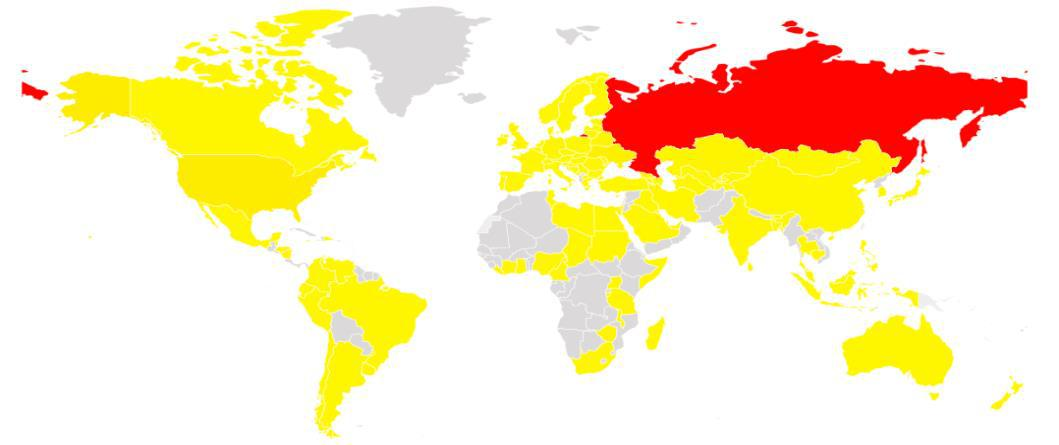
\includegraphics[scale=0.65]{biryulevoDatasetHeatMap}
	}
	\caption{Biryulevo dataset heat map}\label{fig:biryulevoDatasetHeatMap}
\end{figure}

\begin{figure}[ht]
	\centerfloat{
		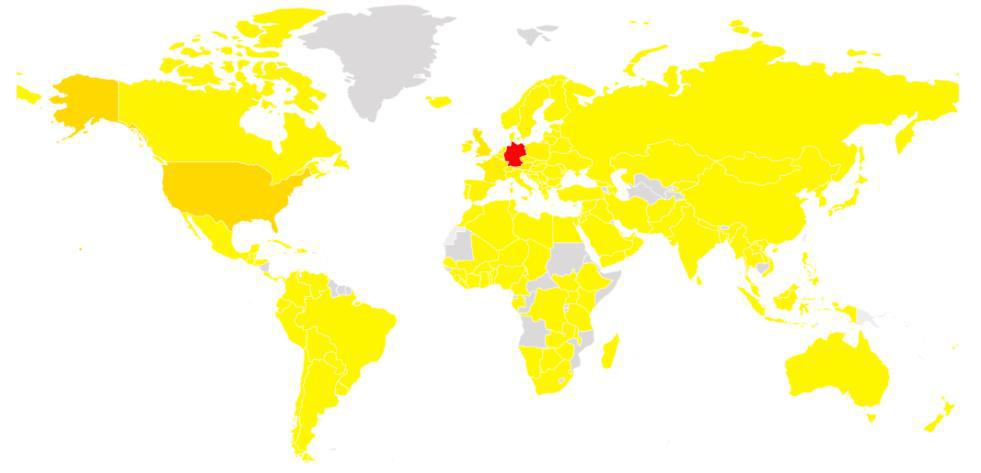
\includegraphics[scale=0.65]{kolnDatasetHeatMap}
	}
	\caption{Köln dataset heat map}\label{fig:kolnDatasetHeatMap}
\end{figure}

\begin{figure}[ht]
	\centerfloat{
		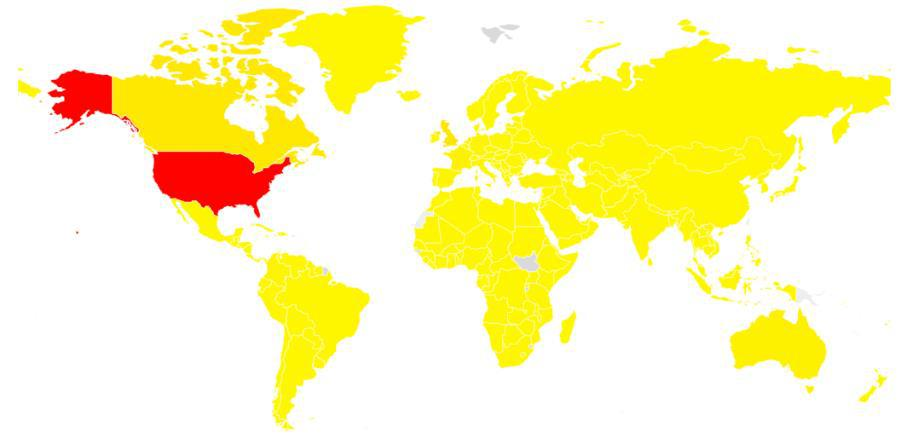
\includegraphics[scale=0.65]{fergusonDatasetHeatMap}
	}
	\caption{Ferguson dataset heat map}\label{fig:fergusonDatasetHeatMap}
\end{figure}

\begin{figure}[ht]
	\centerfloat{
		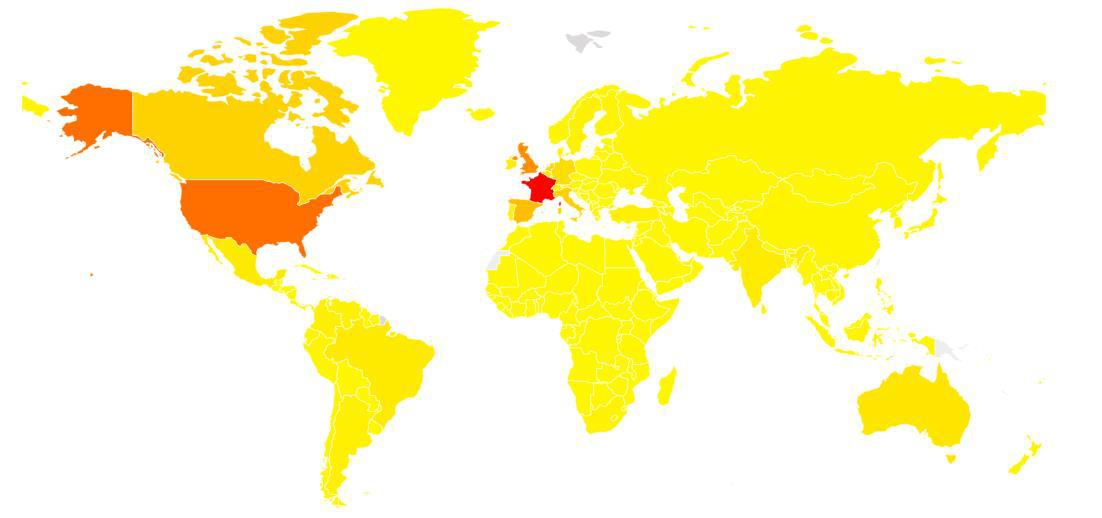
\includegraphics[scale=0.65]{chDatasetHeatMap}
	}
	\caption{«Charlie Hebdo» dataset heat map}\label{fig:chDatasetHeatMap}
\end{figure}

The “naïve+NER+UserGraph” algorithm developed as a result of the study is capable of determining geolocation for users of discussions in social networks who have indicated information about themselves, as well as predicting geolocation for users without such information.

\subsubsection{5 Conclusion}

As a result, authors developed three algorithms “naïve”, “naïve+NER” and “naïve+NER+UserGraph”, which were tested on 4 real user discussions in Twitter social network of different volumes: small size (up to 10 thousand nodes) -- “Biryulyovo”, medium size (up to 50 thousand nodes) -- "Keln”, large size (up to 200 thousand nodes) -- “Ferguson”, extra large size (more than 500 thousand nodes) -- “Charlie Hebdo”.

As a result of the experiment, it was revealed that the \textit{Recall-GEO} measure of the approaches proposed by the authors was quite satisfying: 57\%, 63\% and 76\% for naïve, “naïve+NER” and “naïve+NER+UserGraph” approaches on average, respectively. In particular, the naïve approach allows to determine the geolocation of 57\% of users. NER allows you to refine other 7\% to 12\% for cases when the users specified their geolocation with errors. The graph method allows one to determine location for another 20--23\% of users on top of NER. The latter approach works in cases when the users did not specify their geolocation at all.

Then, we have evaluated the accuracy of the UserGraph method comparing the results of the graph method with the results of other approaches. The final \textit{Precision-GEO} of the UserGraph method turned out to be 72\% on average for the 4 datasets. Taking the simplicity of the latter approach and its decent speed, the evaluated precision value is considered to be good, especially for large-scale discussions.

\section{Сеть маршрутов распространения физических ресурсов на основе данных (обработанных подсетью виртуальных сетевых агентов)}\label{sec:ch6/sect4}

\FloatBarrier

